\documentclass[]{article}
\usepackage{lmodern}
\usepackage{amssymb,amsmath}
\usepackage{ifxetex,ifluatex}
\usepackage{fixltx2e} % provides \textsubscript
\ifnum 0\ifxetex 1\fi\ifluatex 1\fi=0 % if pdftex
  \usepackage[T1]{fontenc}
  \usepackage[utf8]{inputenc}
\else % if luatex or xelatex
  \ifxetex
    \usepackage{mathspec}
  \else
    \usepackage{fontspec}
  \fi
  \defaultfontfeatures{Ligatures=TeX,Scale=MatchLowercase}
\fi
% use upquote if available, for straight quotes in verbatim environments
\IfFileExists{upquote.sty}{\usepackage{upquote}}{}
% use microtype if available
\IfFileExists{microtype.sty}{%
\usepackage{microtype}
\UseMicrotypeSet[protrusion]{basicmath} % disable protrusion for tt fonts
}{}
\usepackage[margin=1in]{geometry}
\usepackage{hyperref}
\hypersetup{unicode=true,
            pdftitle={A3: Modelización predictiva},
            pdfauthor={Paula Muñoz Lago},
            pdfborder={0 0 0},
            breaklinks=true}
\urlstyle{same}  % don't use monospace font for urls
\usepackage{color}
\usepackage{fancyvrb}
\newcommand{\VerbBar}{|}
\newcommand{\VERB}{\Verb[commandchars=\\\{\}]}
\DefineVerbatimEnvironment{Highlighting}{Verbatim}{commandchars=\\\{\}}
% Add ',fontsize=\small' for more characters per line
\usepackage{framed}
\definecolor{shadecolor}{RGB}{248,248,248}
\newenvironment{Shaded}{\begin{snugshade}}{\end{snugshade}}
\newcommand{\AlertTok}[1]{\textcolor[rgb]{0.94,0.16,0.16}{#1}}
\newcommand{\AnnotationTok}[1]{\textcolor[rgb]{0.56,0.35,0.01}{\textbf{\textit{#1}}}}
\newcommand{\AttributeTok}[1]{\textcolor[rgb]{0.77,0.63,0.00}{#1}}
\newcommand{\BaseNTok}[1]{\textcolor[rgb]{0.00,0.00,0.81}{#1}}
\newcommand{\BuiltInTok}[1]{#1}
\newcommand{\CharTok}[1]{\textcolor[rgb]{0.31,0.60,0.02}{#1}}
\newcommand{\CommentTok}[1]{\textcolor[rgb]{0.56,0.35,0.01}{\textit{#1}}}
\newcommand{\CommentVarTok}[1]{\textcolor[rgb]{0.56,0.35,0.01}{\textbf{\textit{#1}}}}
\newcommand{\ConstantTok}[1]{\textcolor[rgb]{0.00,0.00,0.00}{#1}}
\newcommand{\ControlFlowTok}[1]{\textcolor[rgb]{0.13,0.29,0.53}{\textbf{#1}}}
\newcommand{\DataTypeTok}[1]{\textcolor[rgb]{0.13,0.29,0.53}{#1}}
\newcommand{\DecValTok}[1]{\textcolor[rgb]{0.00,0.00,0.81}{#1}}
\newcommand{\DocumentationTok}[1]{\textcolor[rgb]{0.56,0.35,0.01}{\textbf{\textit{#1}}}}
\newcommand{\ErrorTok}[1]{\textcolor[rgb]{0.64,0.00,0.00}{\textbf{#1}}}
\newcommand{\ExtensionTok}[1]{#1}
\newcommand{\FloatTok}[1]{\textcolor[rgb]{0.00,0.00,0.81}{#1}}
\newcommand{\FunctionTok}[1]{\textcolor[rgb]{0.00,0.00,0.00}{#1}}
\newcommand{\ImportTok}[1]{#1}
\newcommand{\InformationTok}[1]{\textcolor[rgb]{0.56,0.35,0.01}{\textbf{\textit{#1}}}}
\newcommand{\KeywordTok}[1]{\textcolor[rgb]{0.13,0.29,0.53}{\textbf{#1}}}
\newcommand{\NormalTok}[1]{#1}
\newcommand{\OperatorTok}[1]{\textcolor[rgb]{0.81,0.36,0.00}{\textbf{#1}}}
\newcommand{\OtherTok}[1]{\textcolor[rgb]{0.56,0.35,0.01}{#1}}
\newcommand{\PreprocessorTok}[1]{\textcolor[rgb]{0.56,0.35,0.01}{\textit{#1}}}
\newcommand{\RegionMarkerTok}[1]{#1}
\newcommand{\SpecialCharTok}[1]{\textcolor[rgb]{0.00,0.00,0.00}{#1}}
\newcommand{\SpecialStringTok}[1]{\textcolor[rgb]{0.31,0.60,0.02}{#1}}
\newcommand{\StringTok}[1]{\textcolor[rgb]{0.31,0.60,0.02}{#1}}
\newcommand{\VariableTok}[1]{\textcolor[rgb]{0.00,0.00,0.00}{#1}}
\newcommand{\VerbatimStringTok}[1]{\textcolor[rgb]{0.31,0.60,0.02}{#1}}
\newcommand{\WarningTok}[1]{\textcolor[rgb]{0.56,0.35,0.01}{\textbf{\textit{#1}}}}
\usepackage{longtable,booktabs}
\usepackage{graphicx,grffile}
\makeatletter
\def\maxwidth{\ifdim\Gin@nat@width>\linewidth\linewidth\else\Gin@nat@width\fi}
\def\maxheight{\ifdim\Gin@nat@height>\textheight\textheight\else\Gin@nat@height\fi}
\makeatother
% Scale images if necessary, so that they will not overflow the page
% margins by default, and it is still possible to overwrite the defaults
% using explicit options in \includegraphics[width, height, ...]{}
\setkeys{Gin}{width=\maxwidth,height=\maxheight,keepaspectratio}
\IfFileExists{parskip.sty}{%
\usepackage{parskip}
}{% else
\setlength{\parindent}{0pt}
\setlength{\parskip}{6pt plus 2pt minus 1pt}
}
\setlength{\emergencystretch}{3em}  % prevent overfull lines
\providecommand{\tightlist}{%
  \setlength{\itemsep}{0pt}\setlength{\parskip}{0pt}}
\setcounter{secnumdepth}{0}
% Redefines (sub)paragraphs to behave more like sections
\ifx\paragraph\undefined\else
\let\oldparagraph\paragraph
\renewcommand{\paragraph}[1]{\oldparagraph{#1}\mbox{}}
\fi
\ifx\subparagraph\undefined\else
\let\oldsubparagraph\subparagraph
\renewcommand{\subparagraph}[1]{\oldsubparagraph{#1}\mbox{}}
\fi

%%% Use protect on footnotes to avoid problems with footnotes in titles
\let\rmarkdownfootnote\footnote%
\def\footnote{\protect\rmarkdownfootnote}

%%% Change title format to be more compact
\usepackage{titling}

% Create subtitle command for use in maketitle
\providecommand{\subtitle}[1]{
  \posttitle{
    \begin{center}\large#1\end{center}
    }
}

\setlength{\droptitle}{-2em}

  \title{A3: Modelización predictiva}
    \pretitle{\vspace{\droptitle}\centering\huge}
  \posttitle{\par}
  \subtitle{Estadística Avanzada, Universitat Oberta de Catalunya}
  \author{Paula Muñoz Lago}
    \preauthor{\centering\large\emph}
  \postauthor{\par}
      \predate{\centering\large\emph}
  \postdate{\par}
    \date{09 diciembre 2019}


\begin{document}
\maketitle

{
\setcounter{tocdepth}{2}
\tableofcontents
}
\hypertarget{modelo-de-regresiuxf3n-lineal}{%
\section{1. Modelo de regresión
lineal}\label{modelo-de-regresiuxf3n-lineal}}

\hypertarget{modelo-de-regresiuxf3n-lineal-simple}{%
\subsection{1.1. Modelo de regresión lineal
simple}\label{modelo-de-regresiuxf3n-lineal-simple}}

\emph{Estimar por mínimos cuadrados ordinarios un modelo lineal que
explique la variable hematocrito en función de la hemoglobina. Evaluar
la bondad de ajuste a través del coeficiente de determinación (R2).
Podéis usar la instrucción de R lm.}

\hypertarget{a-toda-la-muestra-11a}{%
\subsubsection{a) Toda la muestra
\{\#11a\}}\label{a-toda-la-muestra-11a}}

\begin{Shaded}
\begin{Highlighting}[]
\NormalTok{current_working_directory <-}\StringTok{ }\KeywordTok{getwd}\NormalTok{()}
\NormalTok{data <-}\StringTok{ }\KeywordTok{read.csv}\NormalTok{(}\KeywordTok{paste}\NormalTok{(current_working_directory,}\StringTok{"/datosA3.csv"}\NormalTok{, }\DataTypeTok{sep =} \StringTok{""}\NormalTok{))}
\end{Highlighting}
\end{Shaded}

Antes de comenzar, observamos el diagrama de dispersión para las
variables Hematocrito (x) y Hemoglobina (y). Como se puede ver, ambas
variables se encuentran sobre una recta, aunque no se ajustan
perfectamente, con pendiente positiva, que india que a medida que los
Hematocritos aumentan, también lo hace la hemoglobina. Además,
destacamos la presencia de algunos outliers.

\begin{Shaded}
\begin{Highlighting}[]
\KeywordTok{plot}\NormalTok{(data}\OperatorTok{$}\NormalTok{HB, data}\OperatorTok{$}\NormalTok{HCTO)}
\end{Highlighting}
\end{Shaded}

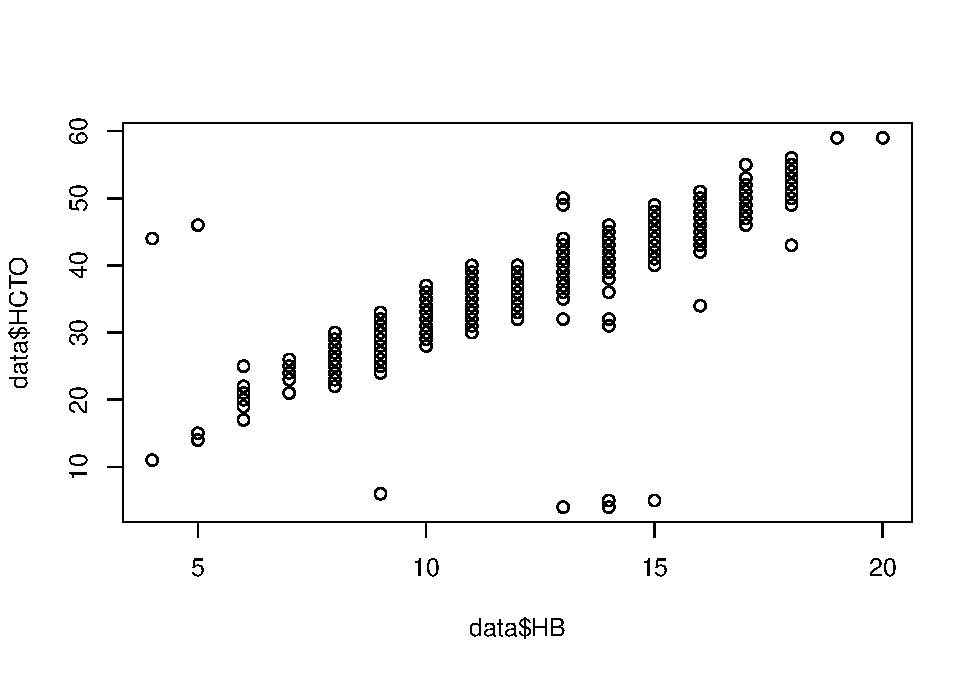
\includegraphics{a3_files/figure-latex/dispersion-1.pdf}

Una vez estudiado el diagrama de dispersión y comprobado que existe una
relación, procedemos a encontrar la ecuación de la recta que mejor se
ajuste a la nube de puntos. La llamaremos la recta de regresión y la
buscaremos con el método de regresión lineal de mínimos cuadrados
ordinarios, que consiste en encontrar una relación entre dos variables
en un plano y minimizar sus residuos, que son la diferencia entre el
valor real y el valor predicho.

\begin{Shaded}
\begin{Highlighting}[]
\NormalTok{model <-}\StringTok{ }\KeywordTok{lm}\NormalTok{(}\DataTypeTok{formula=}\NormalTok{data}\OperatorTok{$}\NormalTok{HCTO }\OperatorTok{~}\StringTok{ }\NormalTok{data}\OperatorTok{$}\NormalTok{HB)}
\KeywordTok{summary}\NormalTok{(model)}
\end{Highlighting}
\end{Shaded}

\begin{verbatim}
## 
## Call:
## lm(formula = data$HCTO ~ data$HB)
## 
## Residuals:
##     Min      1Q  Median      3Q     Max 
## -38.989  -0.989   0.034   1.056  27.636 
## 
## Coefficients:
##             Estimate Std. Error t value Pr(>|t|)    
## (Intercept)  6.31870    0.32991   19.15   <2e-16 ***
## data$HB      2.51136    0.02479  101.31   <2e-16 ***
## ---
## Signif. codes:  0 '***' 0.001 '**' 0.01 '*' 0.05 '.' 0.1 ' ' 1
## 
## Residual standard error: 2.551 on 2341 degrees of freedom
##   (10 observations deleted due to missingness)
## Multiple R-squared:  0.8143, Adjusted R-squared:  0.8142 
## F-statistic: 1.026e+04 on 1 and 2341 DF,  p-value: < 2.2e-16
\end{verbatim}

Una vez construido el modelo, procedemos a visualizar los residuos
generados.

\begin{Shaded}
\begin{Highlighting}[]
\KeywordTok{par}\NormalTok{(}\DataTypeTok{mfrow =} \KeywordTok{c}\NormalTok{(}\DecValTok{2}\NormalTok{, }\DecValTok{2}\NormalTok{))}
\KeywordTok{plot}\NormalTok{(model)}
\end{Highlighting}
\end{Shaded}

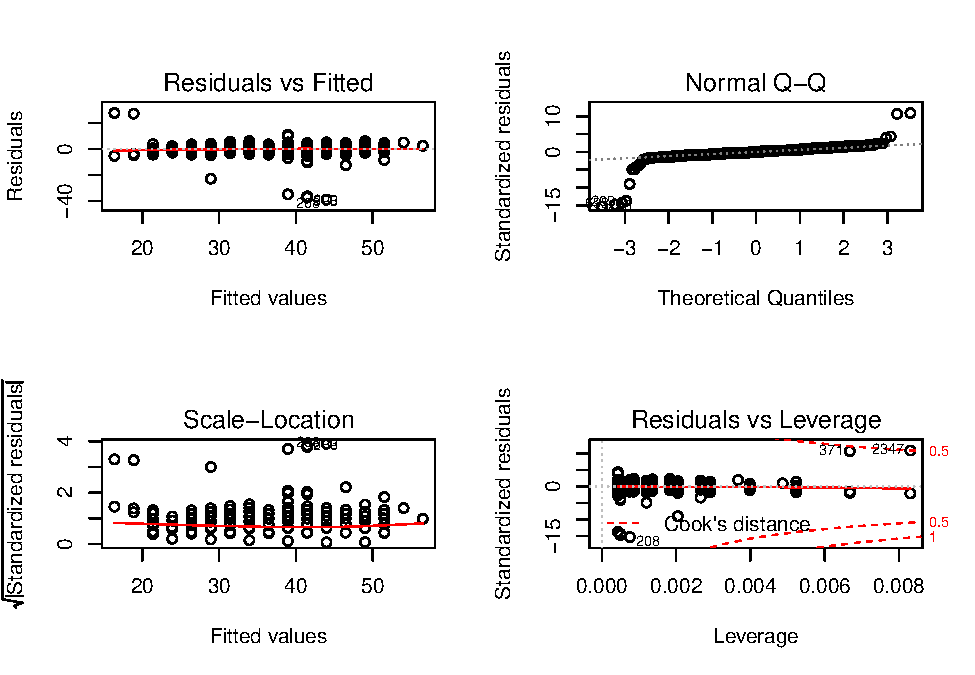
\includegraphics{a3_files/figure-latex/printresiduos-1.pdf}

A continuación, evaluaremos la bondad del ajuste basándonos en el
coeficiente de determinación (R2). Éste nos indica el grado de ajuste de
la recta de regresión a los valores de la muestra.

\begin{Shaded}
\begin{Highlighting}[]
\NormalTok{r2 <-}\StringTok{ }\KeywordTok{summary}\NormalTok{(model)}\OperatorTok{$}\NormalTok{r.squared}
\NormalTok{r2}
\end{Highlighting}
\end{Shaded}

\begin{verbatim}
## [1] 0.8142837
\end{verbatim}

En este caso, el coeficiente de determinación es 0.8142. Dado que r2 = 1
indica un ajuste perfecto, es decrir, todos los puntos se encuentran
sobre la recta de regresión, mientras que r2 = 0 denota la falta de
relación entre los Hematocritos y la Hemoglobina (X e Y
respectivamente). En este caso, dado que r2 se encuentra más cerca de 1,
concluimos que existe una fuerte relación entre ambas variables, sin
llegar a ser un ajuste perfecto.

La recta de regresión lineal obtenida es la siguiente.

\begin{Shaded}
\begin{Highlighting}[]
\KeywordTok{plot}\NormalTok{(data}\OperatorTok{$}\NormalTok{HB, data}\OperatorTok{$}\NormalTok{HCTO)}
\KeywordTok{abline}\NormalTok{(model, }\DataTypeTok{col =} \StringTok{"red"}\NormalTok{)}
\end{Highlighting}
\end{Shaded}

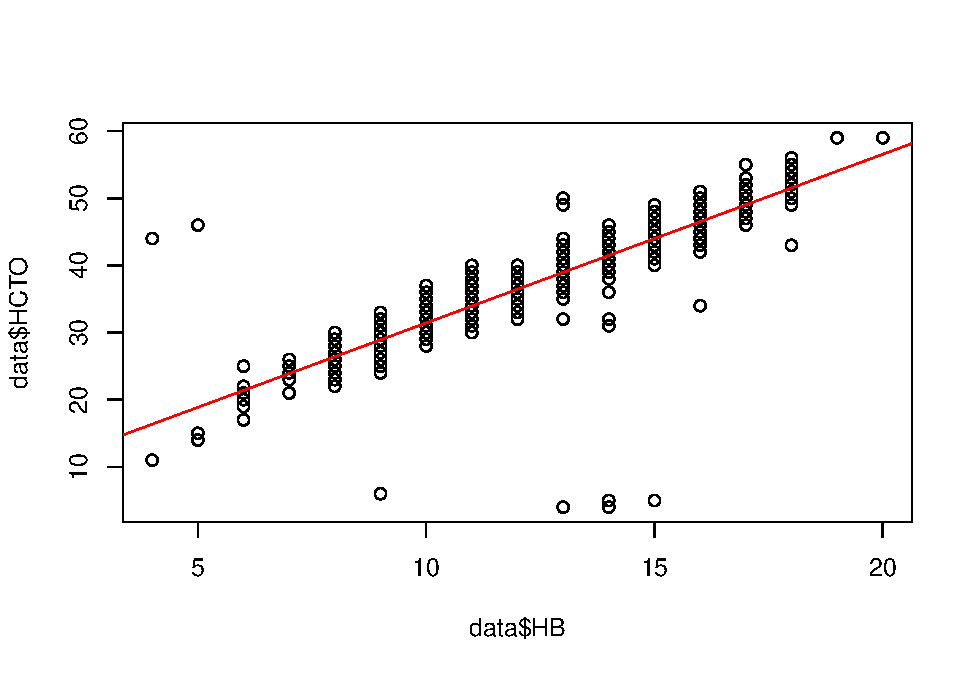
\includegraphics{a3_files/figure-latex/unnamed-chunk-1-1.pdf}

\hypertarget{b-divisiuxf3n-de-la-muestra-en-dos}{%
\subsubsection{b) División de la muestra en
dos}\label{b-divisiuxf3n-de-la-muestra-en-dos}}

\emph{Algunos estudios afirman que la relación calculada anteriormente
varía según la persona esté en condiciones óptimas de salud o no. Para
contestar a esta pregunta, se dividirá la muestra en dos, según si la
persona presenta desnutrición o no. Posteriormente se repetirá el
estudio para cada muestra por separado. A partir de los resultados del
modelo lineal en cada una de las muestras, ¿se puede tomar como cierta
dicha conclusión? Justificar la respuesta.}

En primer lugar, estudiaremos la relación entre os Hematocritos y la
Hemoglobina en personas que presentan desnutrición. Repetiremos el
proceso anterior: tras la división de la muestra, observaremos el
diagrama de dispersión de ambas variables, que, como anteriormente, se
muestran relaionadas en el eje positivo. A continuación, ejecutaremos el
modelo y extraeremos la variable R2.

\begin{Shaded}
\begin{Highlighting}[]
\NormalTok{hcto_desnutri <-}\StringTok{ }\NormalTok{data}\OperatorTok{$}\NormalTok{HCTO[}\KeywordTok{which}\NormalTok{(data}\OperatorTok{$}\NormalTok{DESNUTR }\OperatorTok{==}\StringTok{ "si"}\NormalTok{)]}
\NormalTok{hb_desnutri <-}\StringTok{ }\NormalTok{data}\OperatorTok{$}\NormalTok{HB[}\KeywordTok{which}\NormalTok{(data}\OperatorTok{$}\NormalTok{DESNUTR }\OperatorTok{==}\StringTok{ "si"}\NormalTok{)]}
\NormalTok{model_desnutri <-}\StringTok{ }\KeywordTok{lm}\NormalTok{(hcto_desnutri }\OperatorTok{~}\StringTok{ }\NormalTok{hb_desnutri)}
\NormalTok{r2_desnutri <-}\KeywordTok{summary}\NormalTok{(model_desnutri)}\OperatorTok{$}\NormalTok{r.squared}
\NormalTok{r2_desnutri}
\end{Highlighting}
\end{Shaded}

\begin{verbatim}
## [1] 0.9603207
\end{verbatim}

\begin{Shaded}
\begin{Highlighting}[]
\KeywordTok{plot}\NormalTok{(hb_desnutri, hcto_desnutri)}
\KeywordTok{abline}\NormalTok{(model_desnutri, }\DataTypeTok{col =} \StringTok{"red"}\NormalTok{)}
\end{Highlighting}
\end{Shaded}

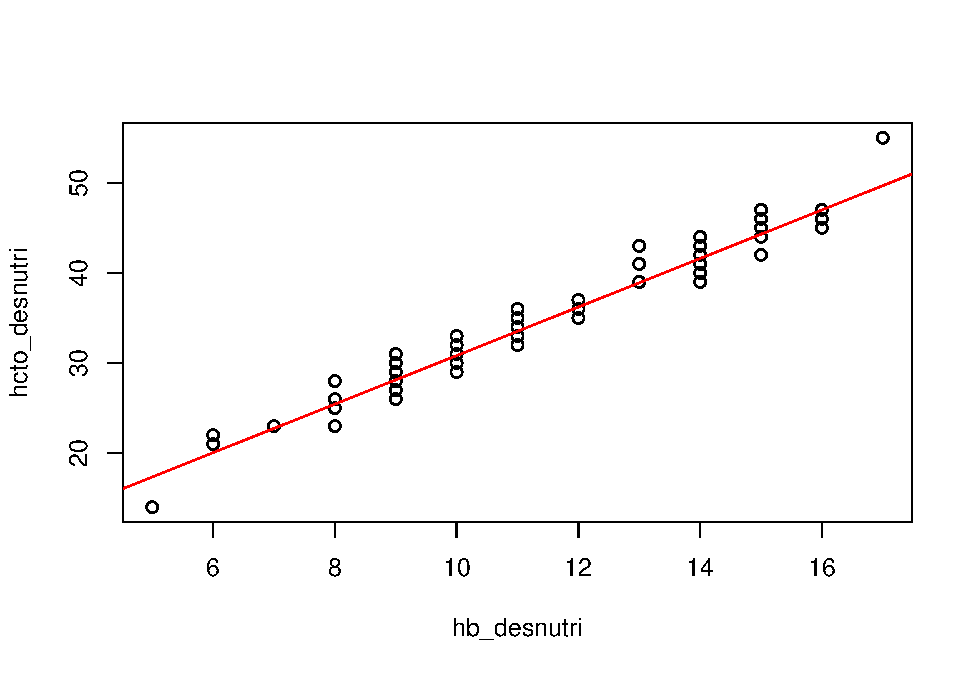
\includegraphics{a3_files/figure-latex/desnutri-1.pdf}

Dado que la variable R2 es muy cercana a 1, podemos concluir que ambas
variables están fuertemente relacionadas en casos de desnutrición.

A continuación, extraeremos del conjunto de datos únicamente a los
individuos que no presentan desnutrición en el momento del estudio. En
este caso, la gráfica de dispersión muestra los valores algo más
distanciados de la recta central, aunque sigue podiendose distinguir
claramente la tendencia a que cuando aumentan los Hematocritos, aumenta
también la Hemoglobina.

\begin{Shaded}
\begin{Highlighting}[]
\NormalTok{hcto_nutri <-}\StringTok{ }\NormalTok{data}\OperatorTok{$}\NormalTok{HCTO[}\KeywordTok{which}\NormalTok{(data}\OperatorTok{$}\NormalTok{DESNUTR }\OperatorTok{==}\StringTok{ "no"}\NormalTok{)]}
\NormalTok{hb_nutri <-}\StringTok{ }\NormalTok{data}\OperatorTok{$}\NormalTok{HB[}\KeywordTok{which}\NormalTok{(data}\OperatorTok{$}\NormalTok{DESNUTR }\OperatorTok{==}\StringTok{ "no"}\NormalTok{)]}
\NormalTok{model_nutri <-}\StringTok{ }\KeywordTok{lm}\NormalTok{(hcto_nutri }\OperatorTok{~}\StringTok{ }\NormalTok{hb_nutri)}
\NormalTok{r2_nutri <-}\KeywordTok{summary}\NormalTok{(model_nutri)}\OperatorTok{$}\NormalTok{r.squared}
\NormalTok{r2_nutri}
\end{Highlighting}
\end{Shaded}

\begin{verbatim}
## [1] 0.7966207
\end{verbatim}

\begin{Shaded}
\begin{Highlighting}[]
\KeywordTok{plot}\NormalTok{(hb_nutri, hcto_nutri)}
\KeywordTok{abline}\NormalTok{(model_nutri, }\DataTypeTok{col =} \StringTok{"red"}\NormalTok{)}
\end{Highlighting}
\end{Shaded}

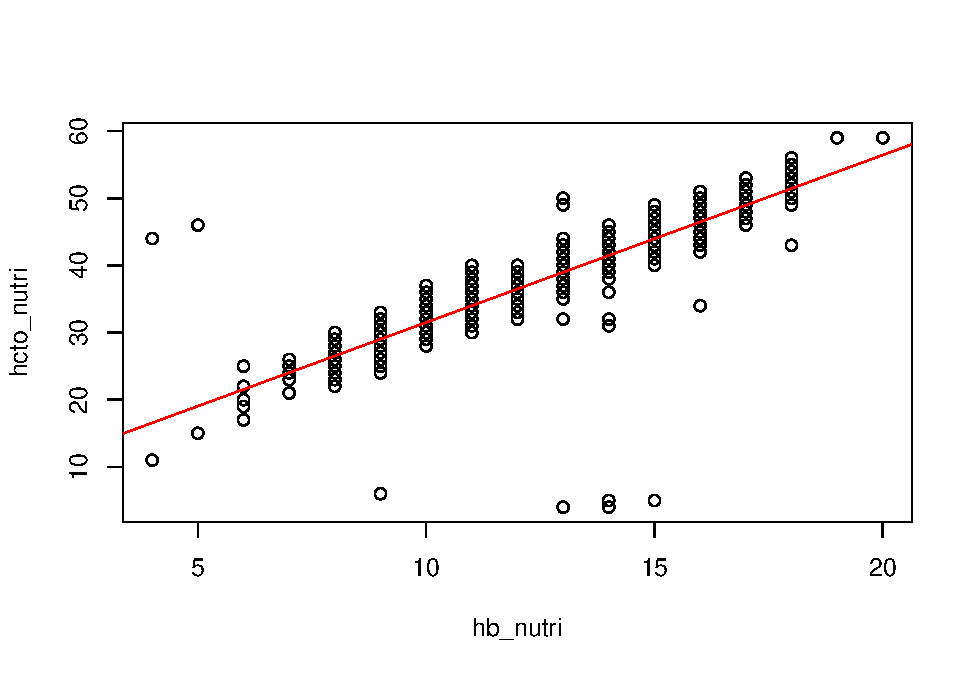
\includegraphics{a3_files/figure-latex/nutri-1.pdf}

Como pudimos preveer en la gráfica de dispersión, los valores X e Y en
el caso de individuos que no presentan desnutrición están menos
relacionados, hemos podido comprobar esta sospecha gracias al valor
r2\_nutri, que es inferior a r2\_desnutri pero igualmente está lo
suficientemente cerca de 1 como para concluir que también existe una
relación entre ambas variables. Es por ello que concluimos que
independientemente de la condición nutricional del individuo, el nivel
de Hematocritos y Hemoblobina estarán relacionados en mayor o menor
medida.

\hypertarget{regresiuxf3n-linear-muxfaltiple-regresores-cuantitativos}{%
\subsection{1.2. Regresión linear múltiple (regresores
cuantitativos)}\label{regresiuxf3n-linear-muxfaltiple-regresores-cuantitativos}}

\begin{Shaded}
\begin{Highlighting}[]
\NormalTok{model_multiple <-}\StringTok{ }\KeywordTok{lm}\NormalTok{(HCTO }\OperatorTok{~}\StringTok{ }\NormalTok{HB }\OperatorTok{+}\StringTok{ }\NormalTok{EDAD, }\DataTypeTok{data=}\NormalTok{data)}
\KeywordTok{summary}\NormalTok{(model_multiple)}
\end{Highlighting}
\end{Shaded}

\begin{verbatim}
## 
## Call:
## lm(formula = HCTO ~ HB + EDAD, data = data)
## 
## Residuals:
##     Min      1Q  Median      3Q     Max 
## -39.188  -1.075   0.006   1.196  27.762 
## 
## Coefficients:
##             Estimate Std. Error t value Pr(>|t|)    
## (Intercept) 5.469021   0.399018  13.706  < 2e-16 ***
## HB          2.533452   0.025430  99.624  < 2e-16 ***
## EDAD        0.010250   0.002706   3.787 0.000156 ***
## ---
## Signif. codes:  0 '***' 0.001 '**' 0.01 '*' 0.05 '.' 0.1 ' ' 1
## 
## Residual standard error: 2.545 on 2338 degrees of freedom
##   (12 observations deleted due to missingness)
## Multiple R-squared:  0.8153, Adjusted R-squared:  0.8152 
## F-statistic:  5162 on 2 and 2338 DF,  p-value: < 2.2e-16
\end{verbatim}

\begin{Shaded}
\begin{Highlighting}[]
\KeywordTok{par}\NormalTok{(}\DataTypeTok{mfrow =} \KeywordTok{c}\NormalTok{(}\DecValTok{2}\NormalTok{, }\DecValTok{2}\NormalTok{))}
\KeywordTok{plot}\NormalTok{(model_multiple)}
\end{Highlighting}
\end{Shaded}

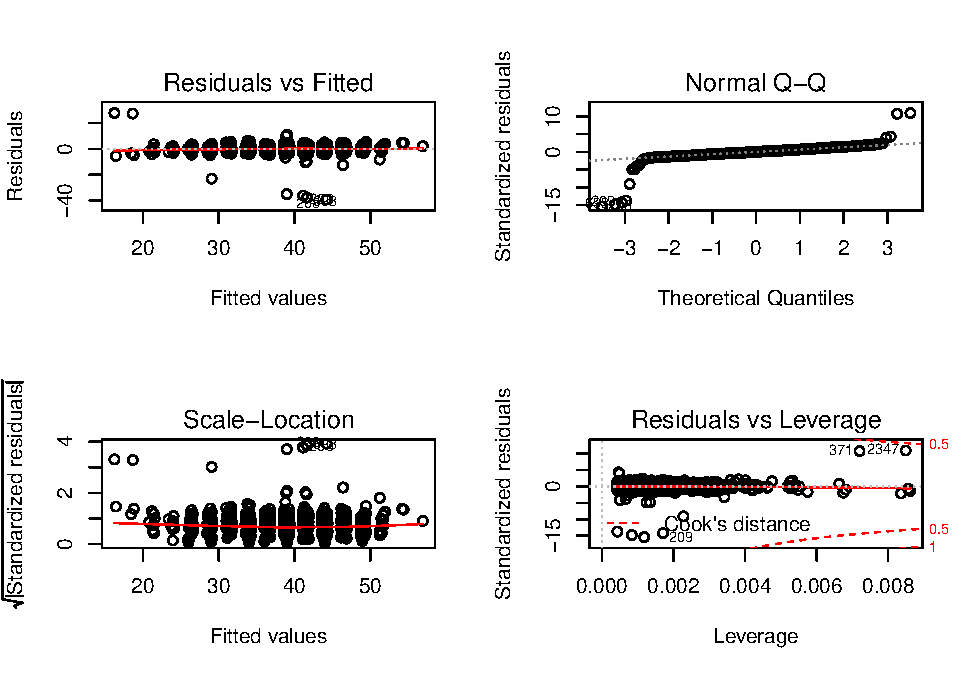
\includegraphics{a3_files/figure-latex/plotmultiple-1.pdf}

Al visualizar estos gráficos se recalca que, dado el primero de ellos,
tenemos una relación linear entre ambas variables, al distribuirse los
residuos sobre la línea horizontal sin patrones aparentes. Según la
segunda gráfica, llamada \emph{Normal Q-Q}, los residuos se distribuyen
siguiente una línea recta, por lo que concluimos que tienen una
distribución normal, pese a los outliers. Dada la gráfica
\emph{Scale-Location}, se asume que tenemos la misma varianza.
Finalmente, la gráfica \emph{Residuals vs Leverage} muestra la
influencia de los outliers en el resultado del análisis dada la
distancia de Cook. Los outliers que encontrasemos fuera de las líneas
punteadas serían influyentes a la hora de obtener la línea de regresión,
pero, dado que en este caso no existen tales valores, concluimos que los
outliers de los que disponemos no alteran el resultado.

\begin{Shaded}
\begin{Highlighting}[]
\NormalTok{r2_multiple <-}\StringTok{ }\KeywordTok{summary}\NormalTok{(model_multiple)}\OperatorTok{$}\NormalTok{r.squared}
\NormalTok{r2_multiple}
\end{Highlighting}
\end{Shaded}

\begin{verbatim}
## [1] 0.8153395
\end{verbatim}

El valor R2 es ligeramente supertior al estudiado en el apartado
\protect\hyperlink{11a}{1.1.a)}, por lo que concluimos que la edad
incrementa levemente la relación entre estas dos variables.

Según los resultados obtenidos en la ejecución de la función
\emph{summary}, la tabla de coeficientes contiene diferente información.
En primer lugar, la columna \emph{Estimate} nos da los valores a, b y c
para completar la fórmula que determina la recta, siendo \(x_1\) el
valor correspondiente a la Hemoglobina y \(x_2\) el valor
correspondiente a la edad.

\[y = a + bx_1 + cx_2\] \[y = 5.46 + 2.53x_1 + 0.01x_2\] A continuación,
encontramos una columna dedicada al error estandar, que indica la
diferencia entre el coeficiente estimado y el valor real. También
encontramos el valor t (e en t-Student) y al p-value, o la probabilidad
de encontrar un valor más alto que t, que en los tres casos es mínimo.

\hypertarget{regresiuxf3n-linear-muxfaltiple-regresores-cuantitativos-y-cualitativos}{%
\subsection{1.3. Regresión linear múltiple (regresores cuantitativos y
cualitativos)}\label{regresiuxf3n-linear-muxfaltiple-regresores-cuantitativos-y-cualitativos}}

\hypertarget{a-todo-el-conjunto}{%
\subsubsection{a) Todo el conjunto}\label{a-todo-el-conjunto}}

En primer lugar, observaremos las relaciones entre las variables.

\begin{Shaded}
\begin{Highlighting}[]
\NormalTok{d_}\DecValTok{3}\NormalTok{ <-}\StringTok{ }\KeywordTok{data.frame}\NormalTok{(data}\OperatorTok{$}\NormalTok{HCTO, data}\OperatorTok{$}\NormalTok{HB, data}\OperatorTok{$}\NormalTok{EDAD, data}\OperatorTok{$}\NormalTok{INFEC)}
\KeywordTok{names}\NormalTok{(d_}\DecValTok{3}\NormalTok{) <-}\StringTok{ }\KeywordTok{c}\NormalTok{(}\StringTok{"HCTO"}\NormalTok{, }\StringTok{"HB"}\NormalTok{, }\StringTok{"EDAD"}\NormalTok{, }\StringTok{"INFEC"}\NormalTok{)}
\KeywordTok{pairs}\NormalTok{(d_}\DecValTok{3}\NormalTok{)}
\end{Highlighting}
\end{Shaded}

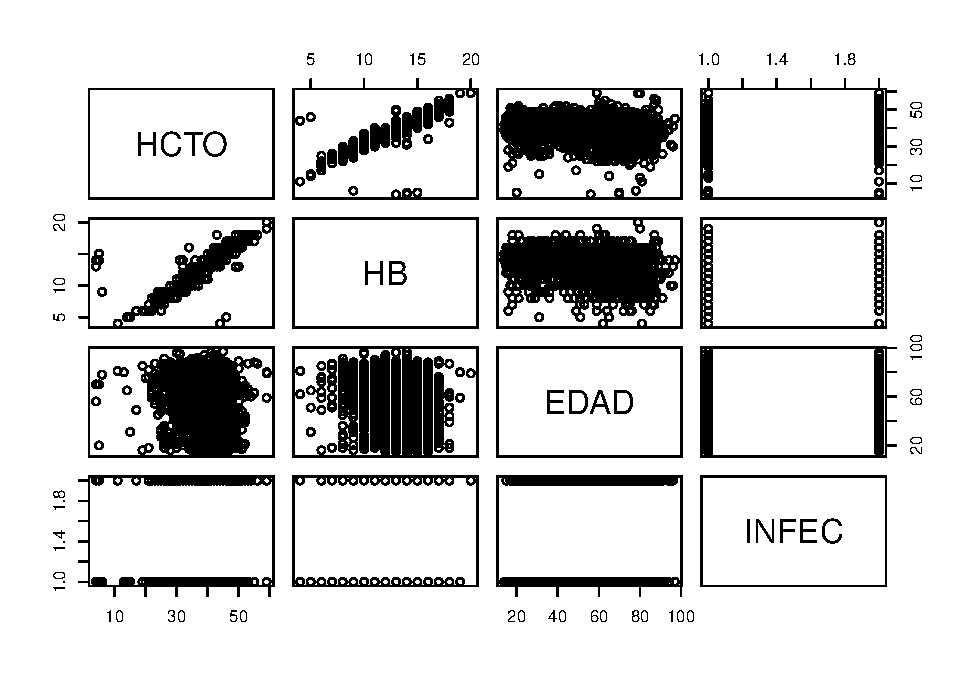
\includegraphics{a3_files/figure-latex/unnamed-chunk-2-1.pdf}

\begin{Shaded}
\begin{Highlighting}[]
\NormalTok{model_multiple_}\DecValTok{2}\NormalTok{ <-}\StringTok{ }\KeywordTok{lm}\NormalTok{(HCTO }\OperatorTok{~}\StringTok{ }\NormalTok{HB }\OperatorTok{+}\StringTok{ }\NormalTok{EDAD }\OperatorTok{+}\StringTok{ }\NormalTok{INFEC, }\DataTypeTok{data=}\NormalTok{data)}
\KeywordTok{summary}\NormalTok{(model_multiple_}\DecValTok{2}\NormalTok{)}
\end{Highlighting}
\end{Shaded}

\begin{verbatim}
## 
## Call:
## lm(formula = HCTO ~ HB + EDAD + INFEC, data = data)
## 
## Residuals:
##     Min      1Q  Median      3Q     Max 
## -39.208  -1.072   0.001   1.186  27.718 
## 
## Coefficients:
##              Estimate Std. Error t value Pr(>|t|)    
## (Intercept)  5.504500   0.401798  13.700  < 2e-16 ***
## HB           2.531145   0.025615  98.816  < 2e-16 ***
## EDAD         0.010525   0.002731   3.854 0.000119 ***
## INFECsi     -0.102044   0.134815  -0.757 0.449173    
## ---
## Signif. codes:  0 '***' 0.001 '**' 0.01 '*' 0.05 '.' 0.1 ' ' 1
## 
## Residual standard error: 2.545 on 2337 degrees of freedom
##   (12 observations deleted due to missingness)
## Multiple R-squared:  0.8154, Adjusted R-squared:  0.8151 
## F-statistic:  3441 on 3 and 2337 DF,  p-value: < 2.2e-16
\end{verbatim}

\begin{Shaded}
\begin{Highlighting}[]
\NormalTok{r2_multiple_}\DecValTok{2}\NormalTok{ <-}\StringTok{ }\KeywordTok{summary}\NormalTok{(model_multiple_}\DecValTok{2}\NormalTok{)}\OperatorTok{$}\NormalTok{r.squared}
\NormalTok{r2_multiple_}\DecValTok{2}
\end{Highlighting}
\end{Shaded}

\begin{verbatim}
## [1] 0.8153848
\end{verbatim}

Como se ha explicado anteriormente, en el resultado de la función
\emph{summary}, en la tabla \emph{Coefficients} encontramos la
estimación de cuanto aumenta o disminuye la variable estudiada en
función de la variable indicada en cada fila. Es decir, por cada unidad
de hemoglobina que aumenta, la cantidad de Hematocritos se incrementa en
un promedio de 2.53. El mismo caso aplica a la edad, que por cada año
que aumenta, la cantidad de hematocritos se incrementa en 0.01. Sin
embargo, al usar variables cualtivativas, se establece que un valor de
referencia, que en este caso es que no haya infección, al que se le
asigna el valor 0, mientras que al otro valor, que sí haya infección, se
le asigna el valor 1. En este caso, indica que el valor de hematocritos
en personas que no presentan infección post-operatoria es 0.1 veces
mayor.
\[NivelHematocritos = 5.5 + 2.53*HB + 0.01*EDAD - 0,1*INFEC_{sí}\] Según
el valor R2 = 0.815, concluimos que las variables están relacionadas.

\hypertarget{b-candidad-de-hematocritos-37}{%
\subsubsection{b) Candidad de Hematocritos \textless{}
37}\label{b-candidad-de-hematocritos-37}}

En primer lugar, observaremos las relaciones entre las variables después
de filtrar según el valor de los hematocritos.

\begin{Shaded}
\begin{Highlighting}[]
\NormalTok{hcto_indexes_less_}\DecValTok{37}\NormalTok{ <-}\StringTok{ }\KeywordTok{which}\NormalTok{(data}\OperatorTok{$}\NormalTok{HCTO }\OperatorTok{<}\StringTok{ }\DecValTok{37}\NormalTok{)}
\NormalTok{d_}\DecValTok{3}\NormalTok{ <-}\StringTok{ }\KeywordTok{data.frame}\NormalTok{(data}\OperatorTok{$}\NormalTok{HCTO[hcto_indexes_less_}\DecValTok{37}\NormalTok{], data}\OperatorTok{$}\NormalTok{HB[hcto_indexes_less_}\DecValTok{37}\NormalTok{], data}\OperatorTok{$}\NormalTok{EDAD[hcto_indexes_less_}\DecValTok{37}\NormalTok{], data}\OperatorTok{$}\NormalTok{INFEC[hcto_indexes_less_}\DecValTok{37}\NormalTok{])}
\KeywordTok{names}\NormalTok{(d_}\DecValTok{3}\NormalTok{) <-}\StringTok{ }\KeywordTok{c}\NormalTok{(}\StringTok{"HCTO"}\NormalTok{, }\StringTok{"HB"}\NormalTok{, }\StringTok{"EDAD"}\NormalTok{, }\StringTok{"INFEC"}\NormalTok{)}
\KeywordTok{pairs}\NormalTok{(d_}\DecValTok{3}\NormalTok{)}
\end{Highlighting}
\end{Shaded}

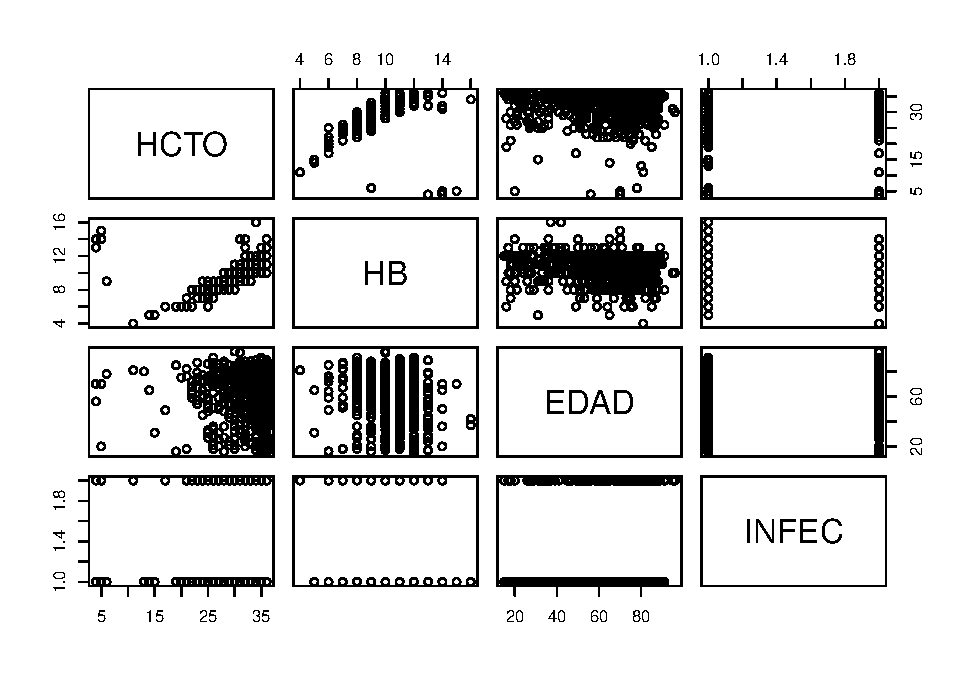
\includegraphics{a3_files/figure-latex/unnamed-chunk-4-1.pdf}

En esta segunda tabla, además de observar una menor densidad en los
gráficos, vemos que los valores de hematocritos se distrubuyen desde 0
hasta el 37, y se puede apreciar cómo, por ejemplo, el gráfico de la
edad, queda \emph{partido} a menos de la mitad que el anterior.
Procedemos a ejecutar el modelo lineal para estudiar la presencia de
relación entre estas variables dada la condición anterior.

\begin{Shaded}
\begin{Highlighting}[]
\NormalTok{hcto_indexes_less_}\DecValTok{37}\NormalTok{ <-}\StringTok{ }\KeywordTok{which}\NormalTok{(data}\OperatorTok{$}\NormalTok{HCTO }\OperatorTok{<}\StringTok{ }\DecValTok{37}\NormalTok{)}
\NormalTok{model_multiple_}\DecValTok{2}\NormalTok{_less37 <-}\StringTok{ }\KeywordTok{lm}\NormalTok{(HCTO }\OperatorTok{~}\StringTok{ }\NormalTok{HB }\OperatorTok{+}\StringTok{ }\NormalTok{EDAD }\OperatorTok{+}\StringTok{ }\NormalTok{INFEC, }\DataTypeTok{data=}\NormalTok{data[hcto_indexes_less_}\DecValTok{37}\NormalTok{,])}
\KeywordTok{summary}\NormalTok{(model_multiple_}\DecValTok{2}\NormalTok{_less37)}
\end{Highlighting}
\end{Shaded}

\begin{verbatim}
## 
## Call:
## lm(formula = HCTO ~ HB + EDAD + INFEC, data = data[hcto_indexes_less_37, 
##     ])
## 
## Residuals:
##     Min      1Q  Median      3Q     Max 
## -35.616  -0.806   0.350   1.450   5.874 
## 
## Coefficients:
##              Estimate Std. Error t value Pr(>|t|)    
## (Intercept) 10.784778   1.103507   9.773   <2e-16 ***
## HB           1.942643   0.086347  22.498   <2e-16 ***
## EDAD         0.009873   0.007430   1.329    0.184    
## INFECsi     -0.252656   0.306318  -0.825    0.410    
## ---
## Signif. codes:  0 '***' 0.001 '**' 0.01 '*' 0.05 '.' 0.1 ' ' 1
## 
## Residual standard error: 3.465 on 612 degrees of freedom
##   (3 observations deleted due to missingness)
## Multiple R-squared:  0.4662, Adjusted R-squared:  0.4635 
## F-statistic: 178.1 on 3 and 612 DF,  p-value: < 2.2e-16
\end{verbatim}

\begin{Shaded}
\begin{Highlighting}[]
\NormalTok{r2_multiple_}\DecValTok{2}\NormalTok{ <-}\StringTok{ }\KeywordTok{summary}\NormalTok{(model_multiple_}\DecValTok{2}\NormalTok{_less37)}\OperatorTok{$}\NormalTok{r.squared}
\NormalTok{r2_multiple_}\DecValTok{2}
\end{Highlighting}
\end{Shaded}

\begin{verbatim}
## [1] 0.4661596
\end{verbatim}

En este caso, no podemos concluir que las variables estén relacionadas.
Podemos concluir que dada la media del nivel de Hematocritos, al extraer
únicamente casos menores a la media, no disponemos de información
suficiente para hacer la regresión lineal, dado que esta condición nos
deja con 619 observaciones frente a las 2353 anteriores.

\hypertarget{predicciuxf3n-de-la-concentraciuxf3n-de-hematocritos}{%
\subsection{1.4. Predicción de la concentración de
hematocritos}\label{predicciuxf3n-de-la-concentraciuxf3n-de-hematocritos}}

Según el primer modelo estudiado en el punto anterior, el nivel de
Hematocritos predicho para una persona de 60 años on infección
postquirúrjuca y un nivel de Hemoglobina de 10.0 es 31.34, mientras que,
según el segundo modelo, elaborado estudiando únicamente los casos en
los que el nivel de hematocritos es menor que 37, la predición resulta
30.55.

\begin{Shaded}
\begin{Highlighting}[]
\NormalTok{new_pacient <-}\StringTok{ }\KeywordTok{data.frame}\NormalTok{(}\DataTypeTok{EDAD =} \DecValTok{60}\NormalTok{, }\DataTypeTok{INFEC =} \StringTok{"si"}\NormalTok{, }\DataTypeTok{HB =} \FloatTok{10.0}\NormalTok{)}
\NormalTok{p <-}\StringTok{ }\KeywordTok{predict}\NormalTok{(model_multiple_}\DecValTok{2}\NormalTok{, new_pacient)}
\NormalTok{p}
\end{Highlighting}
\end{Shaded}

\begin{verbatim}
##        1 
## 31.34539
\end{verbatim}

\begin{Shaded}
\begin{Highlighting}[]
\NormalTok{p2 <-}\StringTok{ }\KeywordTok{predict}\NormalTok{(model_multiple_}\DecValTok{2}\NormalTok{_less37, new_pacient)}
\NormalTok{p2}
\end{Highlighting}
\end{Shaded}

\begin{verbatim}
##        1 
## 30.55095
\end{verbatim}

Dado que el primer modelo dispone de todos los valores, y el segundo
únicamente los individuos con un nivel de hematocritos menor a 37, el
valor predicho será menor que el primero, cuya recta de regresión es más
precisa al disponer de más valores.

\hypertarget{modelo-de-regresiuxf3n-loguxedstica}{%
\section{2. Modelo de regresión
logística}\label{modelo-de-regresiuxf3n-loguxedstica}}

\hypertarget{anuxe1lisis-crudo.-estimaciuxf3n-de-or}{%
\subsection{2.1. Análisis crudo. Estimación de
OR}\label{anuxe1lisis-crudo.-estimaciuxf3n-de-or}}

\hypertarget{a-relaciuxf3n-entre-infecciuxf3n-postquiruxfargica-con-el-resto-de-variables.-estimar-e-interpretar-las-or.-21a}{%
\subsubsection{a) Relación entre infección postquirúrgica con el resto
de variables. Estimar e interpretar las OR.
\{\#21a\}}\label{a-relaciuxf3n-entre-infecciuxf3n-postquiruxfargica-con-el-resto-de-variables.-estimar-e-interpretar-las-or.-21a}}

Para estudiar la relación entre la infección postquirúrgica y el resto
de variables, realizaremos el test chi-cuadrado, que pertenece a las
llamadas pruebas de bondad de ajuste o contraste, y se utiliza para
analizar la relación entre variables nominales o cualitativas. El
estadístico chi-cuadrado tomará el valor 0 si existe una concordancia
perfecta entre las frecuencias observadas de los valores en las tablas
de contingencia, con las frecuencias esperadas, mientras que si existe
una discrepancia entre dichas frecuencias, el estadístico tomará un
valor grande. Se establecerá como hipótesis nula que las variables son
independientes, mientras que la alternativa será que las variables
presentan una dependencia entre ellas. Si el p-valor obtenido en el test
es menor que 0.05, concluiremos que la hipótesis nula es falsa y
aceptaremos la alternativa y viceversa.

Para realizar el estudio, antes de ejecutar el test, estudiaremos la
tabla de contingencias entre ambas variables e imprimiremos un gráfico
que muestra las relaciones entre ambas,para todas las variables
categórigas, y únicamente para una contínua, y a continuación realizar
el test en base a dicha tabla de contingencias.

\begin{Shaded}
\begin{Highlighting}[]
\NormalTok{conting_diab <-}\StringTok{ }\KeywordTok{table}\NormalTok{(data}\OperatorTok{$}\NormalTok{INFEC, data}\OperatorTok{$}\NormalTok{DIABETES)}
\NormalTok{conting_diab}
\end{Highlighting}
\end{Shaded}

\begin{verbatim}
##     
##        no   si
##   no 1792   97
##   si  419   45
\end{verbatim}

\begin{Shaded}
\begin{Highlighting}[]
\NormalTok{conting_desnutri <-}\StringTok{ }\KeywordTok{table}\NormalTok{(data}\OperatorTok{$}\NormalTok{INFEC, data}\OperatorTok{$}\NormalTok{DESNUTR)}
\NormalTok{conting_desnutri}
\end{Highlighting}
\end{Shaded}

\begin{verbatim}
##     
##        no   si
##   no 1831   54
##   si  418   43
\end{verbatim}

\begin{Shaded}
\begin{Highlighting}[]
\NormalTok{conting_obes <-}\StringTok{ }\KeywordTok{table}\NormalTok{(data}\OperatorTok{$}\NormalTok{INFEC, data}\OperatorTok{$}\NormalTok{OBES)}
\NormalTok{conting_obes}
\end{Highlighting}
\end{Shaded}

\begin{verbatim}
##     
##        no   si
##   no 1379  249
##   si  303   99
\end{verbatim}

\begin{Shaded}
\begin{Highlighting}[]
\NormalTok{conting_edad <-}\StringTok{ }\KeywordTok{table}\NormalTok{(data}\OperatorTok{$}\NormalTok{INFEC, data}\OperatorTok{$}\NormalTok{EDAD)}
\KeywordTok{head}\NormalTok{(conting_edad)}
\end{Highlighting}
\end{Shaded}

\begin{verbatim}
##     
##      14 15 16 17 18 19 20 21 22 23 24 25 26 27 28 29 30 31 32 33 34 35 36 37 38
##   no  3 14 22 30 31 24 21 26 17 19 24 18 19 21 19 19 17 24 16 17 15 20 20 16 41
##   si  0  1  0  5  2  1  2  2  3  1  2  6  4  8  3  1  4  3  4  3  4  5  5  5  2
##     
##      39 40 41 42 43 44 45 46 47 48 49 50 51 52 53 54 55 56 57 58 59 60 61 62 63
##   no 22 17 31 19 23 17 23 28 21 26 26 25 34 24 33 29 26 28 28 20 47 41 29 32 44
##   si  1  3  3  2  1  2  3  5  5  6 11  8  4  1  5  6  8  2  1  9  9  8  4 10 17
##     
##      64 65 66 67 68 69 70 71 72 73 74 75 76 77 78 79 80 81 82 83 84 85 86 87 88
##   no 30 33 37 34 50 31 33 40 34 34 34 33 36 26 30 25 20 12 20 18 12 15 13 12  5
##   si  9 12  9 13 14 13 12  8 15 14 17 14 10 15  6 10  7  5  8 11  4  6  4  3  5
##     
##      89 90 91 92 94 95 96 97
##   no  6  2  2  1  2  0  0  1
##   si  3  2  1  0  1  1  2  0
\end{verbatim}

\begin{Shaded}
\begin{Highlighting}[]
\NormalTok{conting_hcto <-}\StringTok{ }\KeywordTok{table}\NormalTok{(data}\OperatorTok{$}\NormalTok{INFEC, data}\OperatorTok{$}\NormalTok{HCTO)}
\KeywordTok{head}\NormalTok{(conting_hcto)}
\end{Highlighting}
\end{Shaded}

\begin{verbatim}
##     
##        4   5   6  11  13  14  15  17  19  20  21  22  23  24  25  26  27  28
##   no   1   1   1   0   1   1   1   0   2   1   2   3   6   5  10  15   9  19
##   si   1   1   0   1   0   0   0   1   0   0   1   2   2   3   7  10   7  13
##     
##       29  30  31  32  33  34  35  36  37  38  39  40  41  42  43  44  45  46
##   no   9  25  24  34  29  42  74 109 106 157 134 165 145 181 115 138 102  85
##   si  12  21  14  14  19  21  21  24  19  21  25  30  21  23  34  19  18  18
##     
##       47  48  49  50  51  52  53  54  55  56  59
##   no  48  36  20   7   8   6   1   0   2   0   2
##   si  10  11   7   4   3   1   2   1   0   1   1
\end{verbatim}

\begin{Shaded}
\begin{Highlighting}[]
\KeywordTok{par}\NormalTok{(}\DataTypeTok{mfrow =} \KeywordTok{c}\NormalTok{(}\DecValTok{2}\NormalTok{, }\DecValTok{2}\NormalTok{))}
\KeywordTok{plot}\NormalTok{(conting_diab, }\DataTypeTok{col =} \KeywordTok{c}\NormalTok{(}\StringTok{"red"}\NormalTok{, }\StringTok{"blue"}\NormalTok{), }\DataTypeTok{main =} \StringTok{"Infección vs diabetes"}\NormalTok{, }\DataTypeTok{xlab =} \StringTok{"Infección", ylab = "}\NormalTok{Diabetes}\StringTok{")}
\StringTok{plot(conting_desnutri, col = c("}\NormalTok{red}\StringTok{", "}\NormalTok{blue}\StringTok{"), main = "}\NormalTok{Infección vs desnutrición", }\DataTypeTok{xlab =} \StringTok{"Infección", ylab = "}\NormalTok{Desnutrición")}
\KeywordTok{plot}\NormalTok{(conting_obes, }\DataTypeTok{col =} \KeywordTok{c}\NormalTok{(}\StringTok{"red"}\NormalTok{, }\StringTok{"blue"}\NormalTok{), }\DataTypeTok{main =} \StringTok{"Infección vs obesidad"}\NormalTok{, }\DataTypeTok{xlab =} \StringTok{"Infección", ylab = "}\NormalTok{Obesidad}\StringTok{")}
\StringTok{plot(conting_edad, col = c("}\NormalTok{red}\StringTok{", "}\NormalTok{blue}\StringTok{"), main = "}\NormalTok{Infección vs edad}\StringTok{", xlab = "}\NormalTok{Infección", }\DataTypeTok{ylab =} \StringTok{"Edad"}\NormalTok{)}
\end{Highlighting}
\end{Shaded}

\includegraphics{a3_files/figure-latex/unnamed-chunk-8-1.pdf}

\begin{Shaded}
\begin{Highlighting}[]
\KeywordTok{chisq.test}\NormalTok{(conting_diab)}
\end{Highlighting}
\end{Shaded}

\begin{verbatim}
## 
##  Pearson's Chi-squared test with Yates' continuity correction
## 
## data:  conting_diab
## X-squared = 12.886, df = 1, p-value = 0.0003311
\end{verbatim}

\begin{Shaded}
\begin{Highlighting}[]
\KeywordTok{chisq.test}\NormalTok{(conting_desnutri)}
\end{Highlighting}
\end{Shaded}

\begin{verbatim}
## 
##  Pearson's Chi-squared test with Yates' continuity correction
## 
## data:  conting_desnutri
## X-squared = 37.419, df = 1, p-value = 9.53e-10
\end{verbatim}

\begin{Shaded}
\begin{Highlighting}[]
\KeywordTok{chisq.test}\NormalTok{(conting_obes)}
\end{Highlighting}
\end{Shaded}

\begin{verbatim}
## 
##  Pearson's Chi-squared test with Yates' continuity correction
## 
## data:  conting_obes
## X-squared = 19.115, df = 1, p-value = 1.231e-05
\end{verbatim}

\begin{Shaded}
\begin{Highlighting}[]
\KeywordTok{chisq.test}\NormalTok{(conting_edad)}
\end{Highlighting}
\end{Shaded}

\begin{verbatim}
## Warning in chisq.test(conting_edad): Chi-squared approximation may be incorrect
\end{verbatim}

\begin{verbatim}
## 
##  Pearson's Chi-squared test
## 
## data:  conting_edad
## X-squared = 144.46, df = 82, p-value = 2.536e-05
\end{verbatim}

\begin{Shaded}
\begin{Highlighting}[]
\KeywordTok{chisq.test}\NormalTok{(conting_hcto)}
\end{Highlighting}
\end{Shaded}

\begin{verbatim}
## Warning in chisq.test(conting_hcto): Chi-squared approximation may be incorrect
\end{verbatim}

\begin{verbatim}
## 
##  Pearson's Chi-squared test
## 
## data:  conting_hcto
## X-squared = 161.68, df = 46, p-value = 8.798e-15
\end{verbatim}

Como podemos observar, el p-valor obtenido en todos los tests resulta
menor que 0.05, por lo que rechazaremos la hipótesis nula, que indica
que las variables son independientes, para concluir en que todas
influyen en la presencia de infecciones.

Para calcular el \emph{Odds Ratio} (OR), que puede ser definido como una
medida de asociación enre variables binarias (sus valores son sí y no, 1
y 0), se deben seguir los pasos siguientes. En primer lugar,
realizaremos el estudio con varias funciones\footnote{\url{https://www.r-bloggers.com/computing-odds-ratios-in-r/}}
, de las que extraeremos el cómputo final. Una OR=1 quiere decir que no
hay asociación entre las variables. Una OR\textless{}1 quiere decir que
el valor con el que se está comparando es un factor de protección frente
a la infección. Por último, una OR\textgreater{}1 indica que la
exposición es un factor de riesgo, tanto mayor cuanto mayor sea el valor
de la OR.

\begin{Shaded}
\begin{Highlighting}[]
\NormalTok{oddsratioWald.proc <-}\StringTok{ }\ControlFlowTok{function}\NormalTok{(n00, n01, n10, n11, }\DataTypeTok{alpha =} \FloatTok{0.05}\NormalTok{)\{}
  \CommentTok{#}
  \CommentTok{#  Compute the odds ratio between two binary variables, x and y,}
  \CommentTok{#  as defined by the four numbers nij:}
  \CommentTok{#}
  \CommentTok{#    n00 = number of cases where x = 0 and y = 0}
  \CommentTok{#    n01 = number of cases where x = 0 and y = 1}
  \CommentTok{#    n10 = number of cases where x = 1 and y = 0}
  \CommentTok{#    n11 = number of cases where x = 1 and y = 1}
  \CommentTok{#}
\NormalTok{  OR <-}\StringTok{ }\NormalTok{(n00 }\OperatorTok{*}\StringTok{ }\NormalTok{n11)}\OperatorTok{/}\NormalTok{(n01 }\OperatorTok{*}\StringTok{ }\NormalTok{n10)}
  \CommentTok{#}
  \CommentTok{#  Compute the Wald confidence intervals:}
  \CommentTok{#}
\NormalTok{  siglog <-}\StringTok{ }\KeywordTok{sqrt}\NormalTok{((}\DecValTok{1}\OperatorTok{/}\NormalTok{n00) }\OperatorTok{+}\StringTok{ }\NormalTok{(}\DecValTok{1}\OperatorTok{/}\NormalTok{n01) }\OperatorTok{+}\StringTok{ }\NormalTok{(}\DecValTok{1}\OperatorTok{/}\NormalTok{n10) }\OperatorTok{+}\StringTok{ }\NormalTok{(}\DecValTok{1}\OperatorTok{/}\NormalTok{n11))}
\NormalTok{  zalph <-}\StringTok{ }\KeywordTok{qnorm}\NormalTok{(}\DecValTok{1} \OperatorTok{-}\StringTok{ }\NormalTok{alpha}\OperatorTok{/}\DecValTok{2}\NormalTok{)}
\NormalTok{  logOR <-}\StringTok{ }\KeywordTok{log}\NormalTok{(OR)}
\NormalTok{  loglo <-}\StringTok{ }\NormalTok{logOR }\OperatorTok{-}\StringTok{ }\NormalTok{zalph }\OperatorTok{*}\StringTok{ }\NormalTok{siglog}
\NormalTok{  loghi <-}\StringTok{ }\NormalTok{logOR }\OperatorTok{+}\StringTok{ }\NormalTok{zalph }\OperatorTok{*}\StringTok{ }\NormalTok{siglog}
  \CommentTok{#}
\NormalTok{  ORlo <-}\StringTok{ }\KeywordTok{exp}\NormalTok{(loglo)}
\NormalTok{  ORhi <-}\StringTok{ }\KeywordTok{exp}\NormalTok{(loghi)}
  \CommentTok{#}
\NormalTok{  oframe <-}\StringTok{ }\KeywordTok{data.frame}\NormalTok{(}\DataTypeTok{LowerCI =}\NormalTok{ ORlo, }\DataTypeTok{OR =}\NormalTok{ OR, }\DataTypeTok{UpperCI =}\NormalTok{ ORhi, }\DataTypeTok{alpha =}\NormalTok{ alpha)}
\NormalTok{  oframe}
\NormalTok{\}}

\NormalTok{AutomaticOR.proc <-}\StringTok{ }\ControlFlowTok{function}\NormalTok{(x,y,}\DataTypeTok{alpha=}\FloatTok{0.05}\NormalTok{)\{}
  \CommentTok{#}
\NormalTok{  xtab <-}\StringTok{ }\KeywordTok{table}\NormalTok{(x,y)}
\NormalTok{  n00 <-}\StringTok{ }\NormalTok{xtab[}\DecValTok{1}\NormalTok{,}\DecValTok{1}\NormalTok{]}
\NormalTok{  n01 <-}\StringTok{ }\NormalTok{xtab[}\DecValTok{1}\NormalTok{,}\DecValTok{2}\NormalTok{]}
\NormalTok{  n10 <-}\StringTok{ }\NormalTok{xtab[}\DecValTok{2}\NormalTok{,}\DecValTok{1}\NormalTok{]}
\NormalTok{  n11 <-}\StringTok{ }\NormalTok{xtab[}\DecValTok{2}\NormalTok{,}\DecValTok{2}\NormalTok{]}
  \CommentTok{#}
\NormalTok{  rawOR <-}\StringTok{ }\NormalTok{(n00}\OperatorTok{*}\NormalTok{n11)}\OperatorTok{/}\NormalTok{(n01}\OperatorTok{*}\NormalTok{n10)}
  \ControlFlowTok{if}\NormalTok{ (rawOR }\OperatorTok{<}\StringTok{ }\DecValTok{1}\NormalTok{)\{}
\NormalTok{    n01 <-}\StringTok{ }\NormalTok{xtab[}\DecValTok{1}\NormalTok{,}\DecValTok{1}\NormalTok{]}
\NormalTok{    n00 <-}\StringTok{ }\NormalTok{xtab[}\DecValTok{1}\NormalTok{,}\DecValTok{2}\NormalTok{]}
\NormalTok{    n11 <-}\StringTok{ }\NormalTok{xtab[}\DecValTok{2}\NormalTok{,}\DecValTok{1}\NormalTok{]}
\NormalTok{    n10 <-}\StringTok{ }\NormalTok{xtab[}\DecValTok{2}\NormalTok{,}\DecValTok{2}\NormalTok{]}
\NormalTok{    iLevel <-}\StringTok{ }\DecValTok{2}
\NormalTok{  \}}
  \ControlFlowTok{else}\NormalTok{\{}
\NormalTok{    iLevel <-}\StringTok{ }\DecValTok{1}
\NormalTok{  \}}
\NormalTok{  outList <-}\StringTok{ }\KeywordTok{vector}\NormalTok{(}\StringTok{"list"}\NormalTok{,}\DecValTok{2}\NormalTok{)}
\NormalTok{  outList[[}\DecValTok{1}\NormalTok{]] <-}\StringTok{ }\KeywordTok{paste}\NormalTok{(}\StringTok{"Odds ratio between the level ["}\NormalTok{,}\KeywordTok{dimnames}\NormalTok{(xtab)[[}\DecValTok{1}\NormalTok{]][}\DecValTok{1}\NormalTok{],}\StringTok{"] of the first variable and the level ["}\NormalTok{,}\KeywordTok{dimnames}\NormalTok{(xtab)[[}\DecValTok{2}\NormalTok{]][iLevel],}\StringTok{"] of the second variable:"}\NormalTok{,}\DataTypeTok{sep=}\StringTok{" "}\NormalTok{)}
\NormalTok{  outList[[}\DecValTok{2}\NormalTok{]] <-}\StringTok{ }\KeywordTok{oddsratioWald.proc}\NormalTok{(n00,n01,n10,n11,alpha)}
\NormalTok{  outList}
\NormalTok{\}}
\end{Highlighting}
\end{Shaded}

De esta manera, al llamar a la última función, obtendremos el valor Odds
para el primer estudio, la relación entre una infección postquirúrgica y
tener diabetes.

\begin{Shaded}
\begin{Highlighting}[]
\KeywordTok{AutomaticOR.proc}\NormalTok{(data}\OperatorTok{$}\NormalTok{INFEC, data}\OperatorTok{$}\NormalTok{DIABETES)}
\end{Highlighting}
\end{Shaded}

\begin{verbatim}
## [[1]]
## [1] "Odds ratio between the level [ no ] of the first variable and the level [ no ] of the second variable:"
## 
## [[2]]
##    LowerCI       OR  UpperCI alpha
## 1 1.371639 1.984106 2.870051  0.05
\end{verbatim}

De esta forma, obtenemos que el \emph{Odds ratio} es 1.984. Así, podemos
proceder con el estudio del resto de variables, a excepción de la edad y
el nivel de hematocritos, cuyo resultado no será relevante dado que no
se trata de variables binarias.

\begin{Shaded}
\begin{Highlighting}[]
\KeywordTok{AutomaticOR.proc}\NormalTok{(data}\OperatorTok{$}\NormalTok{INFEC, data}\OperatorTok{$}\NormalTok{DESNUTR)}
\end{Highlighting}
\end{Shaded}

\begin{verbatim}
## [[1]]
## [1] "Odds ratio between the level [ no ] of the first variable and the level [ no ] of the second variable:"
## 
## [[2]]
##    LowerCI       OR  UpperCI alpha
## 1 2.304606 3.488083 5.279306  0.05
\end{verbatim}

\begin{Shaded}
\begin{Highlighting}[]
\KeywordTok{AutomaticOR.proc}\NormalTok{(data}\OperatorTok{$}\NormalTok{INFEC, data}\OperatorTok{$}\NormalTok{OBES)}
\end{Highlighting}
\end{Shaded}

\begin{verbatim}
## [[1]]
## [1] "Odds ratio between the level [ no ] of the first variable and the level [ no ] of the second variable:"
## 
## [[2]]
##   LowerCI       OR  UpperCI alpha
## 1 1.38965 1.809495 2.356186  0.05
\end{verbatim}

\begin{verbatim}
##   Diabetes Desnutricion Obesidad
## 1     1.98         3.48      1.8
\end{verbatim}

Podemos interpretar los resultados indicando que las tres variables
binarias influyen en la aparición de infecciones postquirúrgicas, siendo
la presencia de desnutrición la más determinante, multiplicando por 3.48
la probabilidad de que aparezca la infección en caso de mostrar
desnutrición.

\hypertarget{b-calculo-de-or-para-variables-contuxednuas}{%
\subsubsection{b) Calculo de OR para variables
contínuas}\label{b-calculo-de-or-para-variables-contuxednuas}}

Dado que la edad y el nivel de hematocritos no son variables binarias,
no podrían seguirse los pasos anteriores, ya que el cálculo del OR
únicamente es válido para tablas de contingencia 2x2. Sin embargo,
haciendo uso de este método, podrá estudiarse la relación entre la
presencia de infección y una cierta edad, o una categorización de
edades.

\hypertarget{c-relaciuxf3n-entre-infecciuxf3n-y-tipo-de-operaciuxf3n}{%
\subsubsection{c) Relación entre infección y tipo de
operación}\label{c-relaciuxf3n-entre-infecciuxf3n-y-tipo-de-operaciuxf3n}}

Al igual que en el caso anterior, no podremos establecer una medida de
relación entre la presencia de infección y el tipo de operación que se
ha llevado a cabo dada la naturaleza del método, al no ser el tipo de
operación una variable binaria. Dado que existen 4 tipos de operaciones,
la tabla de contingencias se mostraría de la siguiente forma.

\begin{verbatim}
##     
##      contam limpia pot_cont sucia
##   no    211    824      607   247
##   si     83     51      146   184
\end{verbatim}

\includegraphics{a3_files/figure-latex/unnamed-chunk-14-1.pdf}

Se puede observar que el tipo de operación que más determina que exista
una infección postquirúrgica es la \emph{sucia}, seguida de la \emph{pot
cont}, \emph{contam} y \emph{limpia} en último lugar.

Existen otras formas de obtener el \emph{Odds Ratio}, sin embargo no son
tan directas como la anterior. Por ejemplo, podemos hacer un modelo de
regresión logística y de sus coeficientes obtener el \emph{Odds ratio}
como vemos a continuación.

\begin{Shaded}
\begin{Highlighting}[]
\NormalTok{model <-}\StringTok{ }\KeywordTok{glm}\NormalTok{(INFEC }\OperatorTok{~}\NormalTok{TIP_OPER, }\DataTypeTok{data=}\NormalTok{data, }\DataTypeTok{family=}\StringTok{"binomial"}\NormalTok{)}
\NormalTok{odds <-}\StringTok{ }\KeywordTok{exp}\NormalTok{(}\KeywordTok{coef}\NormalTok{(model))}
\end{Highlighting}
\end{Shaded}

\begin{longtable}[]{@{}cccc@{}}
\caption{Odds ratio Model}\tabularnewline
\toprule
(Intercept) & TIP\_OPERlimpia & TIP\_OPERpot\_cont &
TIP\_OPERsucia\tabularnewline
\midrule
\endfirsthead
\toprule
(Intercept) & TIP\_OPERlimpia & TIP\_OPERpot\_cont &
TIP\_OPERsucia\tabularnewline
\midrule
\endhead
0.3933649 & 0.157343 & 0.6114607 & 1.893761\tabularnewline
\bottomrule
\end{longtable}

Efectivamente, podemos observar que la variable que presenta una mayor
relación con la presencia de infección es el tipo de operación sucia,
que aumenta 1.89 unidades las posibilidades de generar una infección
tras la operación.

\hypertarget{model-de-regresiuxf3n-loguxedstica}{%
\subsection{2.2. Model de regresión
logística}\label{model-de-regresiuxf3n-loguxedstica}}

La regresión logística forma parte de los llamados modelos lineales
generalizados, que tratan de estimar la probabilidad de que ocurra un
evento binario en base a ciertas variables predictoras. Para realizar el
modelo de regresión logística en R, utilizaremos la función glm (general
lineal models), que se diferencia de la función lm en que hay que
especificar el tipo de familia. En nuestro caso, aplicaremos el modelo a
la variable Infección, que es dicotómica (solo puede adoptar dos
valores), por lo que estableceremos la familia ``binomial''.

\hypertarget{a-infecciuxf3n-y-diabetes}{%
\subsubsection{a) Infección y
diabetes}\label{a-infecciuxf3n-y-diabetes}}

\begin{Shaded}
\begin{Highlighting}[]
\NormalTok{model <-}\StringTok{ }\KeywordTok{glm}\NormalTok{(INFEC }\OperatorTok{~}\StringTok{ }\NormalTok{DIABETES, }\DataTypeTok{data=}\NormalTok{data, }\DataTypeTok{family=}\StringTok{"binomial"}\NormalTok{)}
\KeywordTok{summary}\NormalTok{(model)}
\end{Highlighting}
\end{Shaded}

\begin{verbatim}
## 
## Call:
## glm(formula = INFEC ~ DIABETES, family = "binomial", data = data)
## 
## Deviance Residuals: 
##     Min       1Q   Median       3Q      Max  
## -0.8731  -0.6482  -0.6482  -0.6482   1.8239  
## 
## Coefficients:
##             Estimate Std. Error z value Pr(>|z|)    
## (Intercept) -1.45322    0.05426 -26.780  < 2e-16 ***
## DIABETESsi   0.68517    0.18835   3.638 0.000275 ***
## ---
## Signif. codes:  0 '***' 0.001 '**' 0.01 '*' 0.05 '.' 0.1 ' ' 1
## 
## (Dispersion parameter for binomial family taken to be 1)
## 
##     Null deviance: 2336.5  on 2352  degrees of freedom
## Residual deviance: 2324.3  on 2351  degrees of freedom
## AIC: 2328.3
## 
## Number of Fisher Scoring iterations: 4
\end{verbatim}

La interpretación del modelo es similar al anterior. Se puede observar
que la variable DIABETESsi, tiene un p-valor inferior a 0.05, por lo
que, como anteriormente, concluiremos que la presencia de diabetes
influye en la posible presencia de una infección postquirúrgica. En
cambio, la interpretación de los coeficientes varía ligeramente. Existen
funciones para facilitar la interpretación de los coeficientes,
exponenciandolos, y obteniendo así los \emph{Odds ratio}.

\begin{Shaded}
\begin{Highlighting}[]
\KeywordTok{exp}\NormalTok{(}\KeywordTok{coef}\NormalTok{(model))}
\end{Highlighting}
\end{Shaded}

\begin{verbatim}
## (Intercept)  DIABETESsi 
##    0.233817    1.984106
\end{verbatim}

Esto indica que la presencia de diabetes aumenta en 1.98 unidades la
probabilidad de obtener una infección. Como podemos observar, es el
mismo resultado que obtuvimos en el punto
\protect\hyperlink{21a}{2.1.a}.

\hypertarget{b-infecciuxf3n-diabetes-edad-y-nivel-de-hematocritos}{%
\subsubsection{b) Infección, diabetes, edad y nivel de
hematocritos}\label{b-infecciuxf3n-diabetes-edad-y-nivel-de-hematocritos}}

En este caso, la variable dependiente es dicotómica, mientras que las
variables explicativas son cuantitativa discreta en el caso de la edad,
cualitativa en el caso de la diabetes (sí = 1 y no = 0) y continua en el
caso del nivel de hematocritos.

\begin{Shaded}
\begin{Highlighting}[]
\NormalTok{model2 <-}\StringTok{ }\KeywordTok{glm}\NormalTok{(INFEC }\OperatorTok{~}\StringTok{ }\NormalTok{DIABETES }\OperatorTok{+}\StringTok{ }\NormalTok{EDAD }\OperatorTok{+}\StringTok{ }\NormalTok{HEMAT, }\DataTypeTok{data=}\NormalTok{data, }\DataTypeTok{family=}\StringTok{"binomial"}\NormalTok{)}
\KeywordTok{summary}\NormalTok{(model2)}
\end{Highlighting}
\end{Shaded}

\begin{verbatim}
## 
## Call:
## glm(formula = INFEC ~ DIABETES + EDAD + HEMAT, family = "binomial", 
##     data = data)
## 
## Deviance Residuals: 
##     Min       1Q   Median       3Q      Max  
## -1.1805  -0.7020  -0.5810  -0.4327   2.5107  
## 
## Coefficients:
##              Estimate Std. Error z value Pr(>|z|)    
## (Intercept) -0.814496   0.399414  -2.039   0.0414 *  
## DIABETESsi   0.387511   0.199228   1.945   0.0518 .  
## EDAD         0.018358   0.002986   6.148 7.83e-10 ***
## HEMAT       -0.378479   0.076409  -4.953 7.29e-07 ***
## ---
## Signif. codes:  0 '***' 0.001 '**' 0.01 '*' 0.05 '.' 0.1 ' ' 1
## 
## (Dispersion parameter for binomial family taken to be 1)
## 
##     Null deviance: 2231.4  on 2247  degrees of freedom
## Residual deviance: 2144.3  on 2244  degrees of freedom
##   (105 observations deleted due to missingness)
## AIC: 2152.3
## 
## Number of Fisher Scoring iterations: 4
\end{verbatim}

\begin{Shaded}
\begin{Highlighting}[]
\NormalTok{odds <-}\StringTok{ }\KeywordTok{exp}\NormalTok{(}\KeywordTok{coefficients}\NormalTok{(model2))}
\end{Highlighting}
\end{Shaded}

\begin{longtable}[]{@{}cccc@{}}
\caption{Odds ratio Model2}\tabularnewline
\toprule
(Intercept) & DIABETESsi & EDAD & HEMAT\tabularnewline
\midrule
\endfirsthead
\toprule
(Intercept) & DIABETESsi & EDAD & HEMAT\tabularnewline
\midrule
\endhead
0.4428623 & 1.47331 & 1.018528 & 0.6849025\tabularnewline
\bottomrule
\end{longtable}

En este caso, la variable diabetes deja de ser relevante en la presencia
de infecciones, lo que evidencia este modelo es que la edad y el nivel
de hematocritos es más relevante, es decir, tiene una dependencia más
fuerte a la edad y el nivel de hematocritos que a la diabetes. Como
podemos ver a continuación, esto se debe a que la diabetes sí que está
ligada a la edad, siendo más frecuente en edades más altas. Se puede
observar tanto en el gráfico, como en el resultado del \emph{Odds
range}. Éste es un ejemplo de la paradoja de Simpson.

\begin{Shaded}
\begin{Highlighting}[]
\KeywordTok{plot}\NormalTok{(data}\OperatorTok{$}\NormalTok{EDAD}\OperatorTok{~}\NormalTok{data}\OperatorTok{$}\NormalTok{DIABETES, }\DataTypeTok{ylab=}\StringTok{"EDAD"}\NormalTok{, }\DataTypeTok{xlab=}\StringTok{"DIABETES"}\NormalTok{)}
\end{Highlighting}
\end{Shaded}

\includegraphics{a3_files/figure-latex/unnamed-chunk-21-1.pdf}

\begin{Shaded}
\begin{Highlighting}[]
\NormalTok{model3 <-}\StringTok{ }\KeywordTok{glm}\NormalTok{(DIABETES }\OperatorTok{~}\StringTok{ }\NormalTok{EDAD, }\DataTypeTok{data=}\NormalTok{data, }\DataTypeTok{family=}\StringTok{"binomial"}\NormalTok{)}
\NormalTok{odds <-}\StringTok{ }\KeywordTok{exp}\NormalTok{(}\KeywordTok{coefficients}\NormalTok{(model3))}
\end{Highlighting}
\end{Shaded}

\begin{longtable}[]{@{}cc@{}}
\caption{Odds ratio Model3}\tabularnewline
\toprule
(Intercept) & EDAD\tabularnewline
\midrule
\endfirsthead
\toprule
(Intercept) & EDAD\tabularnewline
\midrule
\endhead
0.0034049 & 1.048615\tabularnewline
\bottomrule
\end{longtable}

Concluiremos con que, teniendo en cuenta la edad y el nivel de
hematocritos, además de la presencia de la enfermedad diabética, diremos
que la diabetes deja de ser tan relevante en la presencia de
infecciones, mientras que la edad y el nivel de hematocritos obtienen un
p-valor menor que 0.05. La presencia de diabetes se mantiene
moderadamente influyente, ya que aumenta 1.47 unidades la probabilidad
de infectarse tras la operación, sin embargo la edad multiplica la
probabilidad por algo más de una unidad por cada año del paciente.
Cuanto menor es el nivel de hematocritos, se aumenta la probabilidad de
subrir una infección en 1.46 puntos, que es la inversa de 0.68.

\hypertarget{mejora-del-modelo}{%
\subsection{2.3. Mejora del modelo}\label{mejora-del-modelo}}

\hypertarget{a-categorizaciuxf3n-variables-continuas}{%
\subsubsection{a) Categorización variables
continuas}\label{a-categorizaciuxf3n-variables-continuas}}

En este caso, convertiremos la edad y el nivel de hematocritos en
variables binarias, dividiendolas en dos agrupaciones, estableceremos el
valor 1 para los casos en los que la edad es mayor o igual a 65, y 0 en
el caso contrario, al igual que estableceremos el valor 1 para los casos
en los que el nivel de hematocritos es superior o igual a 37 y 0 si es
menor.

\begin{Shaded}
\begin{Highlighting}[]
\NormalTok{edad_categorica <-}\StringTok{ }\KeywordTok{c}\NormalTok{()}
\NormalTok{edad_categorica[}\KeywordTok{which}\NormalTok{(data}\OperatorTok{$}\NormalTok{EDAD }\OperatorTok{>=}\StringTok{ }\DecValTok{65}\NormalTok{)] <-}\StringTok{ }\DecValTok{1}
\NormalTok{edad_categorica[}\KeywordTok{which}\NormalTok{(data}\OperatorTok{$}\NormalTok{EDAD }\OperatorTok{<}\StringTok{ }\DecValTok{65}\NormalTok{)] <-}\StringTok{ }\DecValTok{0}
\NormalTok{hematocritos <-}\StringTok{ }\KeywordTok{c}\NormalTok{()}
\NormalTok{hematocritos[}\KeywordTok{which}\NormalTok{(data}\OperatorTok{$}\NormalTok{HCTO }\OperatorTok{>=}\StringTok{ }\DecValTok{37}\NormalTok{)] <-}\StringTok{ }\DecValTok{1}
\NormalTok{hematocritos[}\KeywordTok{which}\NormalTok{(data}\OperatorTok{$}\NormalTok{HCTO }\OperatorTok{<}\StringTok{ }\DecValTok{37}\NormalTok{)] <-}\StringTok{ }\DecValTok{0}

\NormalTok{new_data <-}\StringTok{ }\KeywordTok{data.frame}\NormalTok{(data}\OperatorTok{$}\NormalTok{INFEC, data}\OperatorTok{$}\NormalTok{DIABETES, }\KeywordTok{factor}\NormalTok{(edad_categorica), }\KeywordTok{factor}\NormalTok{(hematocritos))}
\KeywordTok{names}\NormalTok{(new_data) <-}\StringTok{ }\KeywordTok{c}\NormalTok{(}\StringTok{"INFEC"}\NormalTok{, }\StringTok{"DIABETES"}\NormalTok{, }\StringTok{"EDAD_65"}\NormalTok{, }\StringTok{"HCTO_37"}\NormalTok{)}
\KeywordTok{summary}\NormalTok{(new_data)}
\end{Highlighting}
\end{Shaded}

\begin{verbatim}
##  INFEC     DIABETES  EDAD_65     HCTO_37    
##  no:1889   no:2211   0   :1455   0   : 619  
##  si: 464   si: 142   1   : 896   1   :1727  
##                      NA's:   2   NA's:   7
\end{verbatim}

Con este nuevo data frame llamado new\_data, aplicamos el modelo de
regresión logística.

\begin{Shaded}
\begin{Highlighting}[]
\NormalTok{model4 <-}\StringTok{ }\KeywordTok{glm}\NormalTok{(INFEC }\OperatorTok{~}\StringTok{ }\NormalTok{DIABETES }\OperatorTok{+}\StringTok{ }\NormalTok{EDAD_}\DecValTok{65} \OperatorTok{+}\StringTok{ }\NormalTok{HCTO_}\DecValTok{37}\NormalTok{, }\DataTypeTok{data=}\NormalTok{new_data, }\DataTypeTok{family=}\StringTok{"binomial"}\NormalTok{)}
\KeywordTok{summary}\NormalTok{(model4)}
\end{Highlighting}
\end{Shaded}

\begin{verbatim}
## 
## Call:
## glm(formula = INFEC ~ DIABETES + EDAD_65 + HCTO_37, family = "binomial", 
##     data = new_data)
## 
## Deviance Residuals: 
##     Min       1Q   Median       3Q      Max  
## -1.1404  -0.6786  -0.5177  -0.5177   2.0377  
## 
## Coefficients:
##             Estimate Std. Error z value Pr(>|z|)    
## (Intercept)  -1.1459     0.1084 -10.569  < 2e-16 ***
## DIABETESsi    0.4674     0.1946   2.402   0.0163 *  
## EDAD_651      0.5908     0.1086   5.441 5.31e-08 ***
## HCTO_371     -0.7962     0.1115  -7.138 9.46e-13 ***
## ---
## Signif. codes:  0 '***' 0.001 '**' 0.01 '*' 0.05 '.' 0.1 ' ' 1
## 
## (Dispersion parameter for binomial family taken to be 1)
## 
##     Null deviance: 2332.5  on 2343  degrees of freedom
## Residual deviance: 2225.4  on 2340  degrees of freedom
##   (9 observations deleted due to missingness)
## AIC: 2233.4
## 
## Number of Fisher Scoring iterations: 4
\end{verbatim}

\begin{Shaded}
\begin{Highlighting}[]
\NormalTok{odds <-}\StringTok{ }\KeywordTok{exp}\NormalTok{(}\KeywordTok{coefficients}\NormalTok{(model4))}
\end{Highlighting}
\end{Shaded}

\begin{longtable}[]{@{}cccc@{}}
\caption{Odds ratio Model4}\tabularnewline
\toprule
(Intercept) & DIABETESsi & EDAD\_651 & HCTO\_371\tabularnewline
\midrule
\endfirsthead
\toprule
(Intercept) & DIABETESsi & EDAD\_651 & HCTO\_371\tabularnewline
\midrule
\endhead
0.3179474 & 1.595781 & 1.805403 & 0.4510478\tabularnewline
\bottomrule
\end{longtable}

Así, podemos comprobar que la diabetes vuelve a ser más relevante que
anteriormente, siendo su p-valor menor que 0.05, al categorizarse el
resto de variables, y no haber tanta casuística. En este caso la
probabilidad de tener una infección aumenta en casi 1.6 unidades si el
paciente tiene diabetes, así como aumenta en 1.8 si el paciente tiene 65
años o más. Sin embargo, cuanto menor sea el nivel de hematocritos, la
probabilidad de que surga una infección postoperatoria aumenta en 2.21
unidades, que es la inversa de 0.45.

\hypertarget{b-infecciuxf3n-diabetes-edad-nivel-de-hematocritos-y-desnutriciuxf3n}{%
\subsubsection{b) Infección, diabetes, edad, nivel de hematocritos y
desnutrición}\label{b-infecciuxf3n-diabetes-edad-nivel-de-hematocritos-y-desnutriciuxf3n}}

Añadiremos al modelo anterior ya categorizado la variable destrutrición.
En primer lugar, observaremos las gráficas que contienen la relación de
cada variable con la existencia de una futura infección para poder
anticipar qué variables van a ser más significativas.

\begin{Shaded}
\begin{Highlighting}[]
\NormalTok{new_data <-}\StringTok{ }\KeywordTok{data.frame}\NormalTok{(data}\OperatorTok{$}\NormalTok{INFEC, data}\OperatorTok{$}\NormalTok{DIABETES, }\KeywordTok{factor}\NormalTok{(edad_categorica), }\KeywordTok{factor}\NormalTok{(hematocritos), data}\OperatorTok{$}\NormalTok{DESNUTR)}
\KeywordTok{names}\NormalTok{(new_data) <-}\StringTok{ }\KeywordTok{c}\NormalTok{(}\StringTok{"INFEC"}\NormalTok{, }\StringTok{"DIABETES"}\NormalTok{, }\StringTok{"EDAD_65"}\NormalTok{, }\StringTok{"HCTO_37"}\NormalTok{, }\StringTok{"DESNUTR"}\NormalTok{)}
\end{Highlighting}
\end{Shaded}

\includegraphics{a3_files/figure-latex/unnamed-chunk-27-1.pdf}

Como podemos ver, se dan más infecciones en personas diabéticas que las
que no lo son, o en personas de 65 años o mayores. También apreciamos
que la presencia de desnutrición resalta los casos de infección, al
igual que cuando el nivel de hematocritos es menor a 37.

\begin{Shaded}
\begin{Highlighting}[]
\NormalTok{model5 <-}\StringTok{ }\KeywordTok{glm}\NormalTok{(INFEC }\OperatorTok{~}\StringTok{ }\NormalTok{DIABETES }\OperatorTok{+}\StringTok{ }\NormalTok{EDAD_}\DecValTok{65} \OperatorTok{+}\StringTok{ }\NormalTok{HCTO_}\DecValTok{37} \OperatorTok{+}\StringTok{ }\NormalTok{DESNUTR, }\DataTypeTok{data=}\NormalTok{new_data, }\DataTypeTok{family=}\StringTok{"binomial"}\NormalTok{)}
\KeywordTok{summary}\NormalTok{(model5)}
\end{Highlighting}
\end{Shaded}

\begin{verbatim}
## 
## Call:
## glm(formula = INFEC ~ DIABETES + EDAD_65 + HCTO_37 + DESNUTR, 
##     family = "binomial", data = new_data)
## 
## Deviance Residuals: 
##     Min       1Q   Median       3Q      Max  
## -1.4266  -0.6694  -0.5163  -0.5163   2.0402  
## 
## Coefficients:
##             Estimate Std. Error z value Pr(>|z|)    
## (Intercept)  -1.2408     0.1123 -11.052  < 2e-16 ***
## DIABETESsi    0.4463     0.1952   2.286 0.022262 *  
## EDAD_651      0.5661     0.1095   5.171 2.33e-07 ***
## HCTO_371     -0.7071     0.1145  -6.175 6.61e-10 ***
## DESNUTRsi     0.7975     0.2204   3.619 0.000296 ***
## ---
## Signif. codes:  0 '***' 0.001 '**' 0.01 '*' 0.05 '.' 0.1 ' ' 1
## 
## (Dispersion parameter for binomial family taken to be 1)
## 
##     Null deviance: 2321.0  on 2336  degrees of freedom
## Residual deviance: 2204.2  on 2332  degrees of freedom
##   (16 observations deleted due to missingness)
## AIC: 2214.2
## 
## Number of Fisher Scoring iterations: 4
\end{verbatim}

\begin{Shaded}
\begin{Highlighting}[]
\NormalTok{odds <-}\StringTok{ }\KeywordTok{exp}\NormalTok{(}\KeywordTok{coefficients}\NormalTok{(model5))}
\end{Highlighting}
\end{Shaded}

\begin{longtable}[]{@{}ccccc@{}}
\caption{Odds ratio Model5}\tabularnewline
\toprule
(Intercept) & DIABETESsi & EDAD\_651 & HCTO\_371 &
DESNUTRsi\tabularnewline
\midrule
\endfirsthead
\toprule
(Intercept) & DIABETESsi & EDAD\_651 & HCTO\_371 &
DESNUTRsi\tabularnewline
\midrule
\endhead
0.2891641 & 1.562461 & 1.761337 & 0.4930876 & 2.220054\tabularnewline
\bottomrule
\end{longtable}

Podemos observar que en este caso todas las variables observadas son
determinantes en la aparición de futuras infecciones tras una operación.
Los valores presentes en el modelo anterior se mantienen similares,
mientras que la presencia de desnutrición destaca siendo el atributo más
asociado a la aparición de una infección, aumentanto en 2.22 unidades la
probabilidad de que ésta exista.

\hypertarget{predicciuxf3n}{%
\subsection{2.4. Predicción}\label{predicciuxf3n}}

La probabilidad de infectarse para un paciente con las siguientes
características es 0.311.

\begin{Shaded}
\begin{Highlighting}[]
\NormalTok{paciente <-}\StringTok{ }\KeywordTok{data.frame}\NormalTok{(}\DataTypeTok{EDAD_65 =} \KeywordTok{factor}\NormalTok{(}\DecValTok{0}\NormalTok{), }\DataTypeTok{DIABETES =} \StringTok{"si"}\NormalTok{, }\DataTypeTok{HCTO_37 =}\KeywordTok{factor}\NormalTok{(}\DecValTok{0}\NormalTok{), }\DataTypeTok{DESNUTR =} \StringTok{"no"}\NormalTok{)}
\NormalTok{paciente}
\end{Highlighting}
\end{Shaded}

\begin{verbatim}
##   EDAD_65 DIABETES HCTO_37 DESNUTR
## 1       0       si       0      no
\end{verbatim}

\begin{Shaded}
\begin{Highlighting}[]
\KeywordTok{predict}\NormalTok{(model5, paciente, }\DataTypeTok{type =} \StringTok{"response"}\NormalTok{)}
\end{Highlighting}
\end{Shaded}

\begin{verbatim}
##         1 
## 0.3112035
\end{verbatim}

\hypertarget{conclusiones}{%
\subsection{2.5. Conclusiones}\label{conclusiones}}

Finalmente, hemos estudiado varios modelos para establecer una relación
entre variables explicativas y la presencia de una infección
postquirúrgica. De las variables explicativas observadas (EDAD, HCTO,
DESNUTR, DIABETES y TIPO\_OPER), descaca la dependencia de la
desnutrición frente al resto, ya que es la más determinante en la futura
infección. Según se puede ver en el último estudio, aumenta 2.22
unidades la probabilidad de infección. En la siguiente tabla se puede
observar las variables obtenidas en el último modelo ordenadas de menor
a mayor en su nivel de influencia en la presencia de una infección.

\begin{longtable}[]{@{}cccc@{}}
\caption{Summary}\tabularnewline
\toprule
DESNUTRICION\_SI & HCTO\_MENOR\_37 & EDAD\_MAYOR\_65 &
DIABETES\_SI\tabularnewline
\midrule
\endfirsthead
\toprule
DESNUTRICION\_SI & HCTO\_MENOR\_37 & EDAD\_MAYOR\_65 &
DIABETES\_SI\tabularnewline
\midrule
\endhead
2.22 & 2 & 1.76 & 1.56\tabularnewline
\bottomrule
\end{longtable}

Como se ha comentado anteriormente, la presencia de desnutrición es el
atributo del que más depende la presencia de infeccón, seguido del nivel
de hematocritos, que resultara más relevante si es menor. A
continuación, encontramos la edad, que estará más vinculada a la
infección postquirúrgica a medida que aumenta la misma, así como la
presencia de diabetes también es un factor determinante.


\end{document}
